%%PREAMBLE %%%%%%%%%%%%%%%%%%%%%%%%%%%%
\documentclass[10pt, a4paper]{article}% size of txt = 10pt
\usepackage[top= 2cm,
			bottom = 2cm,
			left = 1.7cm,
			right = 1.7cm,
			footskip = 0.5cm,
			headsep = 0cm,
			headheight = 0cm
					]{geometry}
\usepackage{amsmath} % math packages
\usepackage{amsfonts}% math packages
\usepackage{amssymb} % math packages
\usepackage{graphicx} %package for including graphics
\usepackage{array}
\usepackage[thinlines]{easytable}
\usepackage{float}
\usepackage[section]{placeins}
\usepackage[hidelinks]{hyperref}
\usepackage[shortlabels]{enumitem}
\usepackage{svg}
\usepackage{bigstrut}
\usepackage{wrapfig,lipsum,booktabs}
\usepackage{subcaption}
\usepackage{xfrac}
\usepackage{pdfpages}
\usepackage{listings}
\usepackage{xcolor}

\usepackage{listings}
\usepackage{color} %red, green, blue, yellow, cyan, magenta, black, white
\definecolor{mygreen}{RGB}{28,172,0} % color values Red, Green, Blue
\definecolor{mylilas}{RGB}{170,55,241}

\definecolor{codegreen}{rgb}{0,0.6,0}
\definecolor{codegray}{rgb}{0.5,0.5,0.5}
\definecolor{codepurple}{rgb}{0.58,0,0.82}
\definecolor{backcolour}{rgb}{1,1,1}

\lstdefinestyle{mystyle}{
    backgroundcolor=\color{backcolour},   
    commentstyle=\color{codegreen},
    keywordstyle=\color{magenta},
    numberstyle=\tiny\color{codegray},
    stringstyle=\color{codepurple},
    basicstyle=\ttfamily\footnotesize,
    breakatwhitespace=false,         
    breaklines=true,                 
    captionpos=b,                    
    keepspaces=true,                 
    numbers=left,                    
    numbersep=5pt,                  
    showspaces=false,                
    showstringspaces=false,
    showtabs=false,                  
    tabsize=2
}
\lstset{style=mystyle}


%date format
\def\mydate{\leavevmode\hbox{\twodigits\day.\twodigits\month.\the\year}}
\def\twodigits#1{\ifnum#1<10 0\fi\the#1}


\usepackage[T1]{fontenc} 
\usepackage{lmodern}
\usepackage{indentfirst}
\setlength{\parindent}{1cm}

\makeatletter
\newcommand{\thickhline}{%
    \noalign {\ifnum 0=`}\fi \hrule height 2pt
    \futurelet \reserved@a \@xhline
}
\newcolumntype{"}{@{\hskip\tabcolsep\vrule width 2pt\hskip\tabcolsep}}
\makeatother
\newcolumntype{?}{!{\vrule width 2pt}}
%%DOC ENVIROMENT%%%%%%%%%%%%%%%%%%%%%%%
\begin{document}
%Title 
\begin{flushleft}%% left justification
	\textbf{\Large{MKC-KVE: Úloha č. 5}}\hfill Filip Paul\\
	\large{Návrh laseru \hfill\mydate}

\end{flushleft}
\section*{\Large Parametry rezonátoru z předchozího úkolu}
\begin{itemize}
    \item $\gamma_1 = 0\%$
    \item $\gamma_2 = 3\%$
    \item $\gamma_I = 1.3\%$
    \item l = d = 0.111627m
    \item  $\varnothing_1 = \varnothing_2 = 788.95\mu m$ (tady si nejsem jistý, jestli je návrh rezonátoru správný)

\end{itemize}
\section*{\Large Parametry aktivní látky}
\begin{itemize}
    \item $N_\Sigma = 1.6\cdot 10^{25}\,m^{-3}$
    \item $\tau_{21} = 3\,ms$
    \item $\sigma = 2.5\cdot10^{-24}\,m^2$
    \item $lambda_{21}  = 697\,nm$
    \item $w_0 = 0.5\,mm$
    \item $V_f = 0.5\cdot 10^{-8}\,m^{-3}$

    \item Předpokládá se 3 hladinový laser
    \begin{figure}[ht!]
        \centering
        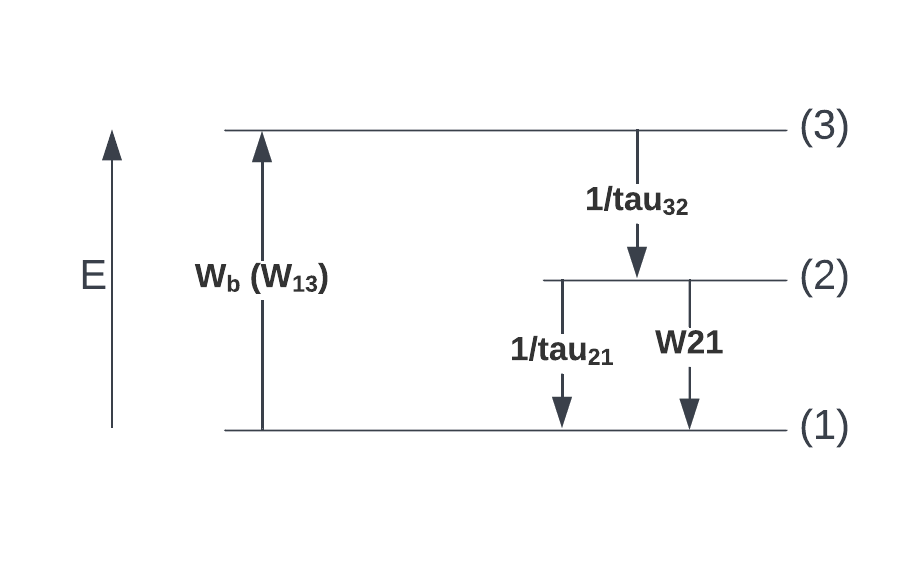
\includegraphics[width=0.5\textwidth]{3hladinovy.png}
    \end{figure}


\end{itemize}
\section*{\Large Výpočty:}
\begin{itemize}
    \item $\Delta N_i^* = \dfrac{(\gamma_1 + \gamma_2)/2+\gamma_i}{\sigma \cdot l} = \dfrac{(0 + 0.03)/2+0.013}{2.5\cdot10^{-24} \cdot 0.111627}
    = 1.034\cdot 10^{23}\,m^{-3}$
    \item $W_b^* = \dfrac{N_\Sigma + \Delta N_i^*}{N_\Sigma - \Delta N_i^*}\cdot \dfrac{1}{\tau_{21}} =
    \dfrac{1.6\cdot 10^{25} + 1.034\cdot 10^{23}}{1.6\cdot 10^{25} - 1.034\cdot 10^{23}}\cdot \dfrac{1}{3\,ms} =337.670\,s^{-1} $
    \item $W_{bmin} = \dfrac{1}{\tau_{21}} = \dfrac{1}{3\,ms} = 333.333\,s^{-1}$
    \clearpage
    \item Závislosti výkonu laseru $P_L$ na buzení $W_b$:
    \item $P_L = \dfrac{V_f\cdot (N_\Sigma +\Delta N_i^*)\cdot \hbar \cdot 2 \cdot \pi \cdot c}{4\cdot \lambda \cdot \tau_{21}}
    \cdot \dfrac{T_2}{\gamma}\cdot\left(\dfrac{W_b}{W_b^*}-1\right)$, kde T2 = $\gamma_2$ a $\gamma = (\gamma_1 + \gamma_2)/2+\gamma_i$\\\\
    Po dosazení $W_b = 2\cdot W_b^*$ do rovnice vychází PL = 2.05028418\,W.
    
    \begin{figure}[ht!]
        \centering
        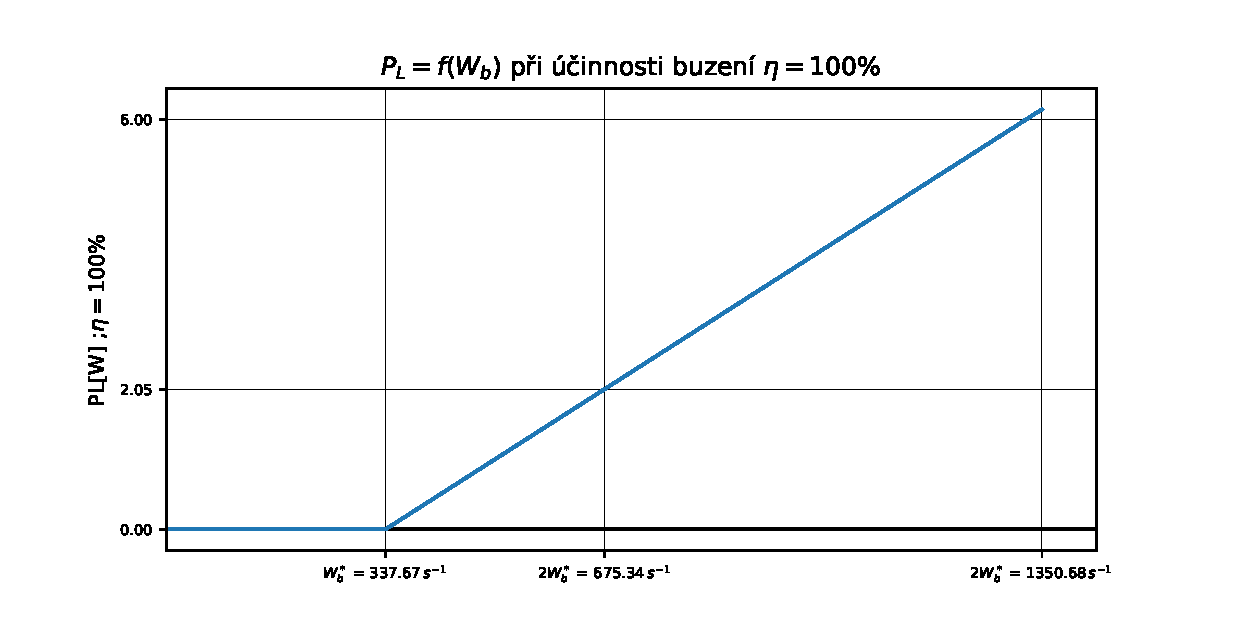
\includegraphics[width=1\textwidth]{graphs.eps}
    \end{figure}
    \item Závislost inverzního počtu částic $\Delta N_i$ na buzení $W_b$:

    \begin{figure}[ht!]
        \centering
        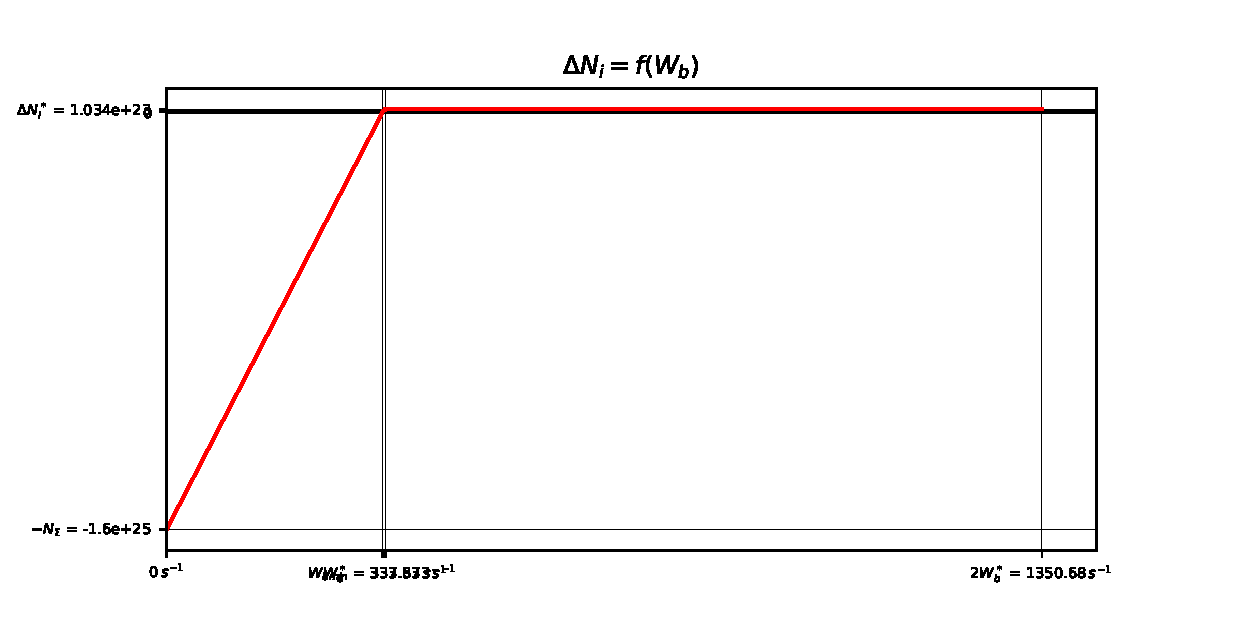
\includegraphics[width=1\textwidth]{N_graph.eps}
    \end{figure}
Pro lepší zobrazení části grafu, kde se počet částic blíží k nule a $\Delta N_i^*$,
je na další stránce zoom tohoto grafu.
    \begin{figure}[ht!]
        \centering
        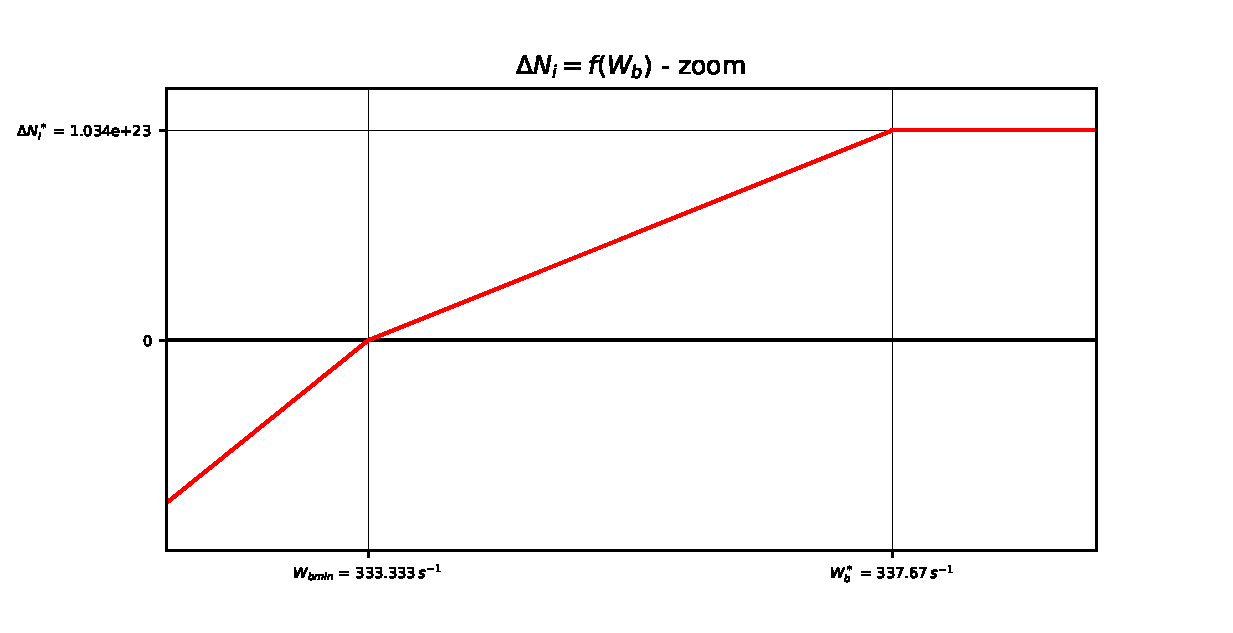
\includegraphics[width=1\textwidth]{N_graph_zoom.eps}
    \end{figure}
\end{itemize}

\section*{\Large Závěr:}
Navrhovaný laser má nevýhodu ve volbě 3 hladinového systému. V tomto systému je oproti 4 hladinovému
systému nutno dodat potřebné množství energie, abychom nejprve dosáhli $\Delta N = 0$. Toto množství energie
odpovídá rychlosti buzení $W_{bmin} = 333.333s^{-1}$. Výhodou by mohla být jednoduchost návrhu. Dále
nevím, jak se pohybuje cena aktivní látky, ale předpokládám, že by 3 hladinový laser mohl být levnější
a výrobně jednodušší ?.

\end{document}

%\[f(x)= (x+2)^2 - \frac{9\cdot 2\pi}{26}\] %%mathematic equatation in display style mode
%%optional:
%	\begin{align} %%this alignes all charakters after & if *is removed equations will be numbered
%	\hspace{5cm}  
%		 x &= a_2 x^2 +_1 x + a_0 \\
% 		x &=x^2 \nonumber		%no number will not add number to eq
%	\end{align}


